\documentclass{article}
\usepackage[utf8]{inputenc}
%\StopShownPreambleCommands
\usepackage{pgfplots}
\usepackage{tikz}
\usepackage{comment}
%\usepackage{arrows}

\title{twikz_plots_DL}


\usepackage{graphicx}

\begin{document}

\tikzstyle{neuron}=[circle,draw=red!50,fill=red!10, thick,minimum size=10mm]
\tikzstyle{neuron1}=[circle,draw=blue!50,fill=cyan!10, thick,minimum size=10mm]
\begin{tikzpicture}
\node [neuron] (neuron1) at (10,0) {};

\draw[->] (neuron1) -- (5.7,1.9);
\draw[->] (neuron1) -- (7.7,1.9);
\node[text width=0.5cm] at (10,1.2) {\LARGE {.}};
\node[text width=0.5cm] at (10.5,1.2) {\LARGE {.}};
\node[text width=0.5cm] at (11,1.2) {\LARGE {.}};
\draw[->] (neuron1) -- (12.7,1.9);
\draw[->] (neuron1) -- (14.7,1.9);

\node[text width=0.5cm] at (5.5,2.5) {Tower maker};
\draw[gray,thick,solid] (5,2) rectangle (6.5,3);

\node[text width=0.5cm] at (7.5,2.5) {Tower maker};
\draw[gray,thick,solid] (7,2) rectangle (8.5,3);

\node[text width=0.5cm] at (9.5,2.5) {\LARGE {.}};
\node[text width=0.5cm] at (10.5,2.5) {\LARGE {.}};
\node[text width=0.5cm] at (11.5,2.5) {\LARGE {.}};

\node[text width=0.5cm] at (12.5,2.5) {Tower maker};
\node[text width=0.5cm] at (12.5,2.5) {Tower maker};

\node[text width=0.5cm] at (12.5,2.5) {Tower maker};
\draw[gray,thick,solid] (12,2) rectangle (13.5,3);

\node[text width=0.5cm] at (14.5,2.5) {Tower maker};
\draw[gray,thick,solid] (14,2) rectangle (15.5,3);

\node (plot) at (5.7,4) {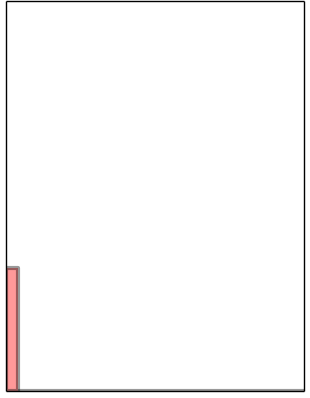
\includegraphics[width=1.7cm,height=1.5cm]{p1.png}};
\node (plot) at (7.7,4) {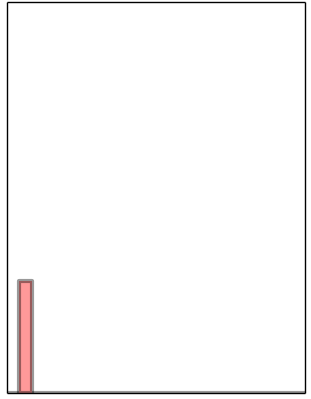
\includegraphics[width=1.7cm,height=1.5cm]{p2.png}};
\node[text width=0.5cm] at (9.5,4) {\LARGE {.}};
\node[text width=0.5cm] at (10.5,4) {\LARGE {.}};
\node[text width=0.5cm] at (11.5,4) {\LARGE {.}};
\node (plot) at (12.7,4) {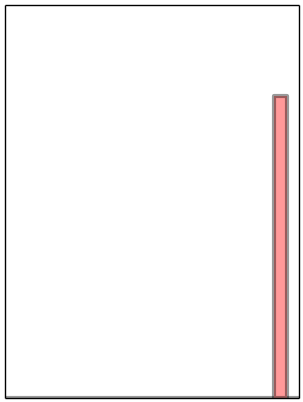
\includegraphics[width=1.7cm,height=1.5cm]{p3.png}};
\node (plot) at (14.7,4) {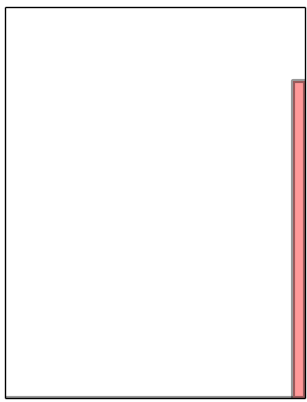
\includegraphics[width=1.7cm,height=1.5cm]{p4.png}};

\node [neuron1] (neuron2) at (10,7) {};
\draw[->]  (5.7,4.8) -- (neuron2);
\draw[->]  (7.7,4.8) -- (neuron2);

\node[text width=0.5cm] at (9.5,5.5) {\LARGE {.}};
\node[text width=0.5cm] at (10.5,5.5) {\LARGE {.}};
\node[text width=0.5cm] at (11.5,5.5) {\LARGE {.}};

\draw[->]  (12.7,4.8) -- (neuron2);
\draw[->]  (14.7,4.8) -- (neuron2);
\node (plot) at (10,9.5) {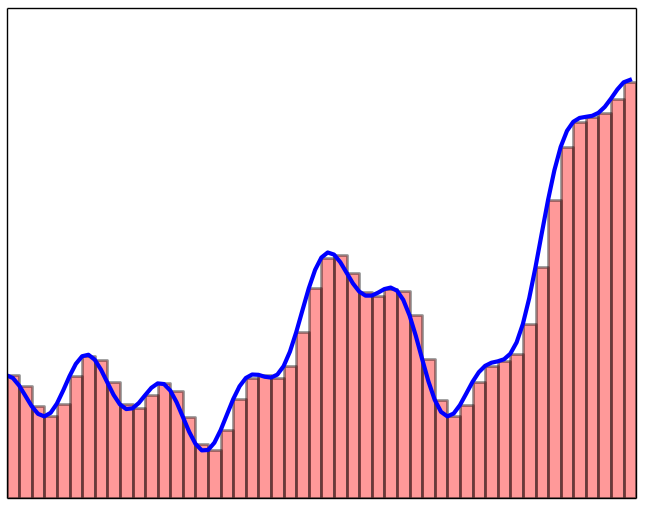
\includegraphics[width=11cm, height=3cm]{plot.png}};

\end{tikzpicture}

\end{document}
